\chapter{The Guests}

In the house in the Rue du Helder, where Albert had invited the Count
of Monte Cristo, everything was being prepared on the morning of the
21st of May to do honor to the occasion. Albert de Morcerf inhabited a
pavilion situated at the corner of a large court, and directly opposite
another building, in which were the servants’ apartments. Two windows
only of the pavilion faced the street; three other windows looked into
the court, and two at the back into the garden.

Between the court and the garden, built in the heavy style of the
imperial architecture, was the large and fashionable dwelling of the
Count and Countess of Morcerf.

A high wall surrounded the whole of the property, surmounted at
intervals by vases filled with flowers, and broken in the centre by a
large gate of gilded iron, which served as the carriage entrance. A
small door, close to the lodge of the \textit{concierge}, gave ingress and
egress to the servants and masters when they were on foot.

It was easy to discover that the delicate care of a mother, unwilling
to part from her son, and yet aware that a young man of the viscount’s
age required the full exercise of his liberty, had chosen this
habitation for Albert. There were not lacking, however, evidences of
what we may call the intelligent egoism of a youth who is charmed with
the indolent, careless life of an only son, and who lives as it were in
a gilded cage. By means of the two windows looking into the street,
Albert could see all that passed; the sight of what is going on is
necessary to young men, who always want to see the world traverse their
horizon, even if that horizon is only a public thoroughfare. Then,
should anything appear to merit a more minute examination, Albert de
Morcerf could follow up his researches by means of a small gate,
similar to that close to the \textit{concierge’s} door, and which merits a
particular description.

It was a little entrance that seemed never to have been opened since
the house was built, so entirely was it covered with dust and dirt; but
the well-oiled hinges and locks told quite another story. This door was
a mockery to the \textit{concierge}, from whose vigilance and jurisdiction it
was free, and, like that famous portal in the \textit{Arabian Nights}, opening
at the “\textit{Sesame}” of Ali Baba, it was wont to swing backward at a
cabalistic word or a concerted tap from without from the sweetest
voices or whitest fingers in the world.

At the end of a long corridor, with which the door communicated, and
which formed the antechamber, was, on the right, Albert’s
breakfast-room, looking into the court, and on the left the salon,
looking into the garden. Shrubs and creeping plants covered the
windows, and hid from the garden and court these two apartments, the
only rooms into which, as they were on the ground floor, the prying
eyes of the curious could penetrate.

On the floor above were similar rooms, with the addition of a third,
formed out of the antechamber; these three rooms were a salon, a
boudoir, and a bedroom. The salon downstairs was only an Algerian
divan, for the use of smokers. The boudoir upstairs communicated with
the bedchamber by an invisible door on the staircase; it was evident
that every precaution had been taken. Above this floor was a large
\textit{atelier}, which had been increased in size by pulling down the
partitions—a pandemonium, in which the artist and the dandy strove for
pre-eminence.

There were collected and piled up all Albert’s successive caprices,
hunting-horns, bass-viols, flutes—a whole orchestra, for Albert had had
not a taste but a fancy for music; easels, palettes, brushes,
pencils—for music had been succeeded by painting; foils, boxing-gloves,
broadswords, and single-sticks—for, following the example of the
fashionable young men of the time, Albert de Morcerf cultivated, with
far more perseverance than music and drawing, the three arts that
complete a dandy’s education, i.e., fencing, boxing, and single-stick;
and it was here that he received Grisier, Cooks, and Charles Leboucher.

The rest of the furniture of this privileged apartment consisted of old
cabinets, filled with Chinese porcelain and Japanese vases, Lucca della
Robbia \textit{faïences}, and Palissy platters; of old armchairs, in which
perhaps had sat Henry IV. or Sully, Louis XIII. or Richelieu—for two of
these armchairs, adorned with a carved shield, on which were engraved
the fleur-de-lis of France on an azure field, evidently came from the
Louvre, or, at least, some royal residence.

Over these dark and sombre chairs were thrown splendid stuffs, dyed
beneath Persia’s sun, or woven by the fingers of the women of Calcutta
or of Chandernagor. What these stuffs did there, it was impossible to
say; they awaited, while gratifying the eyes, a destination unknown to
their owner himself; in the meantime they filled the place with their
golden and silky reflections.

In the centre of the room was a Roller and Blanchet “baby grand” piano
in rosewood, but holding the potentialities of an orchestra in its
narrow and sonorous cavity, and groaning beneath the weight of the
\textit{chefs-d’œuvre} of Beethoven, Weber, Mozart, Haydn, Grétry, and
Porpora.

On the walls, over the doors, on the ceiling, were swords, daggers,
Malay creeses, maces, battle-axes; gilded, damasked, and inlaid suits
of armor; dried plants, minerals, and stuffed birds, their
flame-colored wings outspread in motionless flight, and their beaks
forever open. This was Albert’s favorite lounging place.

However, the morning of the appointment, the young man had established
himself in the small salon downstairs. There, on a table, surrounded at
some distance by a large and luxurious divan, every species of tobacco
known,—from the yellow tobacco of Petersburg to the black of Sinai, and
so on along the scale from Maryland and Porto Rico, to Latakia,—was
exposed in pots of crackled earthenware of which the Dutch are so fond;
beside them, in boxes of fragrant wood, were ranged, according to their
size and quality, puros, regalias, havanas, and manillas; and, in an
open cabinet, a collection of German pipes, of chibouques, with their
amber mouth-pieces ornamented with coral, and of narghiles, with their
long tubes of morocco, awaiting the caprice or the sympathy of the
smokers.

Albert had himself presided at the arrangement, or, rather, the
symmetrical derangement, which, after coffee, the guests at a breakfast
of modern days love to contemplate through the vapor that escapes from
their mouths, and ascends in long and fanciful wreaths to the ceiling.

At a quarter to ten, a valet entered; he composed, with a little groom
named John, and who only spoke English, all Albert’s establishment,
although the cook of the hotel was always at his service, and on great
occasions the count’s \textit{chasseur} also. This valet, whose name was
Germain, and who enjoyed the entire confidence of his young master,
held in one hand a number of papers, and in the other a packet of
letters, which he gave to Albert. Albert glanced carelessly at the
different missives, selected two written in a small and delicate hand,
and enclosed in scented envelopes, opened them and perused their
contents with some attention.

“How did these letters come?” said he.

“One by the post, Madame Danglars’ footman left the other.”

“Let Madame Danglars know that I accept the place she offers me in her
box. Wait; then, during the day, tell Rosa that when I leave the Opera
I will sup with her as she wishes. Take her six bottles of different
wine—Cyprus, sherry, and Malaga, and a barrel of Ostend oysters; get
them at Borel’s, and be sure you say they are for me.”

“At what o’clock, sir, do you breakfast?”

\begin{figure}[ht]
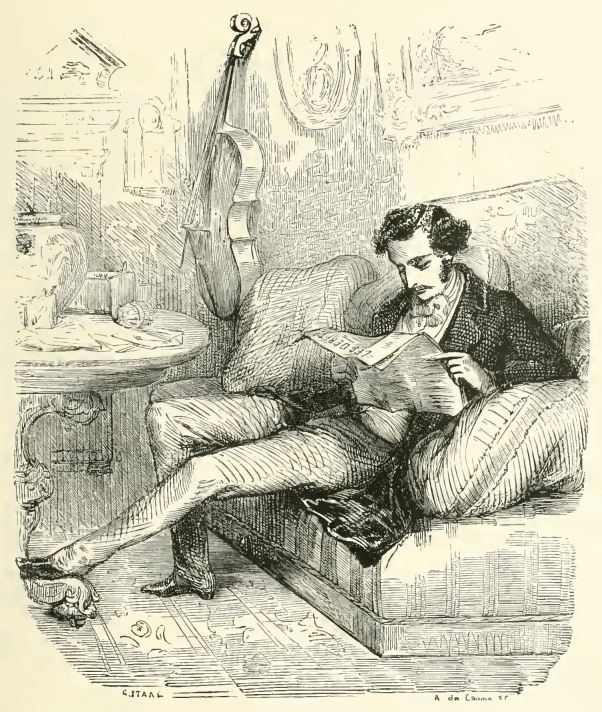
\includegraphics[width=\textwidth]{20227m.jpg}
\end{figure}

“What time is it now?”

“A quarter to ten.”

“Very well, at half past ten. Debray will, perhaps, be obliged to go to
the minister—and besides” (Albert looked at his tablets), “it is the
hour I told the count, 21st May, at half past ten; and though I do not
much rely upon his promise, I wish to be punctual. Is the countess up
yet?”

“If you wish, I will inquire.”

“Yes, ask her for one of her \textit{liqueur} cellarets, mine is incomplete;
and tell her I shall have the honor of seeing her about three o’clock,
and that I request permission to introduce someone to her.”

The valet left the room. Albert threw himself on the divan, tore off
the cover of two or three of the papers, looked at the theatre
announcements, made a face seeing they gave an opera, and not a ballet;
hunted vainly amongst the advertisements for a new tooth-powder of
which he had heard, and threw down, one after the other, the three
leading papers of Paris, muttering,

“These papers become more and more stupid every day.”

A moment after, a carriage stopped before the door, and the servant
announced M. Lucien Debray. A tall young man, with light hair, clear
gray eyes, and thin and compressed lips, dressed in a blue coat with
beautifully carved gold buttons, a white neckcloth, and a tortoiseshell
eye-glass suspended by a silken thread, and which, by an effort of the
superciliary and zygomatic muscles, he fixed in his eye, entered, with
a half-official air, without smiling or speaking.

“Good-morning, Lucien, good-morning,” said Albert; “your punctuality
really alarms me. What do I say? punctuality! You, whom I expected
last, you arrive at five minutes to ten, when the time fixed was
half-past! Has the ministry resigned?”

“No, my dear fellow,” returned the young man, seating himself on the
divan; “reassure yourself; we are tottering always, but we never fall,
and I begin to believe that we shall pass into a state of immobility,
and then the affairs of the Peninsula will completely consolidate us.”

“Ah, true; you drive Don Carlos out of Spain.”

“No, no, my dear fellow, do not confound our plans. We take him to the
other side of the French frontier, and offer him hospitality at
Bourges.”

“At Bourges?”

“Yes, he has not much to complain of; Bourges is the capital of Charles
VII. Do you not know that all Paris knew it yesterday, and the day
before it had already transpired on the Bourse, and M. Danglars (I do
not know by what means that man contrives to obtain intelligence as
soon as we do) made a million!”

“And you another order, for I see you have a blue ribbon at your
button-hole.”

“Yes; they sent me the order of Charles III.,” returned Debray
carelessly.

“Come, do not affect indifference, but confess you were pleased to have
it.”

“Oh, it is very well as a finish to the toilet. It looks very neat on a
black coat buttoned up.”

“And makes you resemble the Prince of Wales or the Duke of Reichstadt.”

“It is for that reason you see me so early.”

“Because you have the order of Charles III., and you wish to announce
the good news to me?”

“No, because I passed the night writing letters,—five-and-twenty
despatches. I returned home at daybreak, and strove to sleep; but my
head ached and I got up to have a ride for an hour. At the Bois de
Boulogne, \textit{ennui} and hunger attacked me at once,—two enemies who
rarely accompany each other, and who are yet leagued against me, a sort
of Carlo-republican alliance. I then recollected you gave a breakfast
this morning, and here I am. I am hungry, feed me; I am bored, amuse
me.”

“It is my duty as your host,” returned Albert, ringing the bell, while
Lucien turned over, with his gold-mounted cane, the papers that lay on
the table. “Germain, a glass of sherry and a biscuit. In the meantime,
my dear Lucien, here are cigars—contraband, of course—try them, and
persuade the minister to sell us such instead of poisoning us with
cabbage leaves.”

“\textit{Peste!} I will do nothing of the kind; the moment they come from
government you would find them execrable. Besides, that does not
concern the home but the financial department. Address yourself to M.
Humann, section of the indirect contributions, corridor A., No. 26.”

“On my word,” said Albert, “you astonish me by the extent of your
knowledge. Take a cigar.”

“Really, my dear Albert,” replied Lucien, lighting a manilla at a
rose-colored taper that burnt in a beautifully enamelled stand—“how
happy you are to have nothing to do. You do not know your own good
fortune!”

“And what would you do, my dear diplomatist,” replied Morcerf, with a
slight degree of irony in his voice, “if you did nothing? What? private
secretary to a minister, plunged at once into European cabals and
Parisian intrigues; having kings, and, better still, queens, to
protect, parties to unite, elections to direct; making more use of your
cabinet with your pen and your telegraph than Napoleon did of his
battle-fields with his sword and his victories; possessing
five-and-twenty thousand francs a year, besides your place; a horse,
for which Château-Renaud offered you four hundred louis, and which you
would not part with; a tailor who never disappoints you; with the
opera, the jockey-club, and other diversions, can you not amuse
yourself? Well, I will amuse you.”

“How?”

“By introducing to you a new acquaintance.”

“A man or a woman?”

“A man.”

“I know so many men already.”

“But you do not know this man.”

“Where does he come from—the end of the world?”

“Farther still, perhaps.”

“The deuce! I hope he does not bring our breakfast with him.”

“Oh, no; our breakfast comes from my father’s kitchen. Are you hungry?”

“Humiliating as such a confession is, I am. But I dined at M. de
Villefort’s, and lawyers always give you very bad dinners. You would
think they felt some remorse; did you ever remark that?”

“Ah, depreciate other persons’ dinners; you ministers give such
splendid ones.”

“Yes; but we do not invite people of fashion. If we were not forced to
entertain a parcel of country boobies because they think and vote with
us, we should never dream of dining at home, I assure you.”

“Well, take another glass of sherry and another biscuit.”

“Willingly. Your Spanish wine is excellent. You see we were quite right
to pacify that country.”

“Yes; but Don Carlos?”

“Well, Don Carlos will drink Bordeaux, and in ten years we will marry
his son to the little queen.”

“You will then obtain the Golden Fleece, if you are still in the
ministry.”

“I think, Albert, you have adopted the system of feeding me on smoke
this morning.”

“Well, you must allow it is the best thing for the stomach; but I hear
Beauchamp in the next room; you can dispute together, and that will
pass away the time.”

“About what?”

“About the papers.”

“My dear friend,” said Lucien with an air of sovereign contempt, “do I
ever read the papers?”

“Then you will dispute the more.”

“M. Beauchamp,” announced the servant. “Come in, come in,” said Albert,
rising and advancing to meet the young man. “Here is Debray, who
detests you without reading you, so he says.”

“He is quite right,” returned Beauchamp; “for I criticise him without
knowing what he does. Good-day, commander!”

“Ah, you know that already,” said the private secretary, smiling and
shaking hands with him.

“\textit{Pardieu!}”

“And what do they say of it in the world?”

“In which world? we have so many worlds in the year of grace 1838.”

“In the entire political world, of which you are one of the leaders.”

“They say that it is quite fair, and that sowing so much red, you ought
to reap a little blue.”

“Come, come, that is not bad!” said Lucien. “Why do you not join our
party, my dear Beauchamp? With your talents you would make your fortune
in three or four years.”

“I only await one thing before following your advice; that is, a
minister who will hold office for six months. My dear Albert, one word,
for I must give poor Lucien a respite. Do we breakfast or dine? I must
go to the Chamber, for our life is not an idle one.”

“You only breakfast; I await two persons, and the instant they arrive
we shall sit down to table.”
